\documentclass[10pt]{llncs} % <<<

\usepackage{amsmath}
\usepackage{amssymb}
%\usepackage{amsthm}
\usepackage{graphics}
\usepackage[latin1]{inputenc}
\usepackage{microtype}  % do not remove
\usepackage{pygmentize}
\usepackage{rgalg}
\usepackage{tikz}
\usepackage{xcolor}
\usepackage{xspace}

\usepackage[colorlinks]{hyperref} % keep it last to avoid some warnings

\RecustomVerbatimEnvironment{Verbatim}{BVerbatim}{}
\definecolor{darkred}{rgb}{0.4,0,0}
\definecolor{darkblue}{rgb}{0,0,0.4}
\definecolor{verylightgray}{rgb}{0.9,0.9,0.9}
\definecolor{lightblue}{rgb}{0,0,0.9}
% comment the next line for printing
\hypersetup{colorlinks,linkcolor=darkblue,citecolor=darkblue,urlcolor=darkblue}
%\hypersetup{
%  pdftitle={TOPL: A Language for Specifying Safety Temporal Properties of Object-Oriented Programs},
%  pdfauthor={Radu Grigore and Rasmus Lerchedahl Petersen and Dino Distefano}}

\newcommand{\TPL}{TOPL}

%\titlebanner{DRAFT}
%\title{Dynamic Checking of Temporal Safety properties for Java}
%\author{\IEEEauthorblockN{Dino Distefano}
%\IEEEauthorblockA{Queen Mary University of London\\
%ddino@eecs.qmul.ac.uk}
%\and
%\IEEEauthorblockN{Radu Grigore}
%\IEEEauthorblockA{Queen Mary University of London\\
% rgrig@eecs.qmul.ac.uk}
% \and%
%\IEEEauthorblockN{Rasmus Lerchedahl Petersen}
%\IEEEauthorblockA{Queen Mary University of London\\
% rusmus@eecs.qmul.ac.uk}
%}

\title{Dynamic Checking of Temporal Safety properties for Java}
\author{Dino Distefano \and Radu Grigore \and Rasmus Lerchedahl Petersen}


\institute{Queen Mary University of London }
 

% rg: I tend to give grammars in BFS order
\def\grammar#1{{
  \footnotesize
  \def\b##1{{\rm\Verb@##1@}}\def\*{$^*$}\def\?{$^?$}\def\({$($}\def\){$)$}
  \def\|{$\mid$}\def\+{$^+$}
  \smallskip
  \hbox to\hsize{\hfil\vbox{\halign{\hfil\it##&$\;::=\;$\it##\hfil&\qquad\rm##\hfil\cr#1}}\hfil}
  \smallskip
}}

\renewcommand{\sectionautorefname}{Section}
\renewcommand{\subsectionautorefname}{\sectionautorefname}

\newcommand{\noterg}[2]{\textcolor{gray}{[\textcolor{red}{#1}: #2]}}
%\renewcommand{\note}[2]{}
\newcommand{\rg}[1]{\noterg{rg}{#1}}
\newcommand{\rlp}[1]{\noterg{rlp}{#1}}
\newcommand{\dd}[1]{\noterg{dd}{#1}}
\newcommand{\dinocomment}[1]{\dd{#1}}

\newcommand{\B}{\ensuremath{\mathbb{B}}}
\newcommand{\N}{\ensuremath{\mathbb{N}}}
\newcommand{\delimitVerbatim}{\par\nobreak\smallskip\noindent}
\newcommand{\error}{\ensuremath{\textcolor{darkred}{\mathtt{error}}}\xspace}
\newcommand{\eval}[1]{[[#1]]}
\newcommand{\pattern}[1]{\ensuremath{\mathtt{\underline{#1}}}}
\newcommand{\pmap}{\rightharpoonup}
\newcommand{\set}[1]{\ensuremath{\mathsf{#1}}}
\newcommand{\start}{\ensuremath{\mathtt{start}}\xspace}
\newcommand{\verbline}[2][]{\[\text{\Verb@#2@}#1\]}

\newcommand{\functionfont}[1]{\mathit{#1}}
\newcommand{\desugar}{\functionfont{des}}
\newcommand{\enabled}{\functionfont{enabled}}

\newcommand{\codefont}[1]{\mathtt{#1}}
\newcommand{\this}{\codefont{this}}

%\theoremstyle{definition}
%\newtheorem{example}{Example}
%\theoremstyle{remark}
%\newtheorem{remark}{Remark}
\newtheorem{notation}{Notation}

%\overfullrule=5pt
%\showboxdepth=10
%\showboxbreadth=30
% >>>
\begin{document}
\maketitle

\begin{abstract} % <<<
In this paper we introduce a new technique for checking, at run-time, temporal safety properties for Java programs.
Our technique is based on a new general specification language which is able to express complex properties of 
systems involving various objects. The specifications are then used to instrument byte-code  so that violations of the specifications can be automatically detected at run-time. 
We have experimented our technique by checking several safety properties on large open source projects.
\end{abstract}
%\begin{IEEEkeywords}
%Safety, Temporal Properties, Object-Oriented, Dynamic Checking
%\end{IEEEkeywords}

%\category{D.2.1}{Software Engineering}{Requirements/Specifications}
%\terms Languages, Verification
%\keywords Safety, Temporal Properties, Object-Oriented

% >>>
\section{Introduction} % <<<

Objects interaction is at the core of the object-oriented paradigm. When designing object-oriented software, 
programmers have often  a global picture of the co-operation that objects will have in different moments and the 
invariants that all the player should adhere to for the correct functioning of the system.
These invariants are often naturally expressible as {\em temporal safety properties} which, in turn, have been 
studied in several contexts by the formal methods and the verification community. 
%
%The verification community showed interest in \emph{safety temporal properties} for a long time.
%Manna and Pnueli~\cite{dblp:books/daglib/0080029} provide a theoretical foundation and clearly argue why such %properties are crucial.
In this article, we focus on the automatic dynamic checking of safety temporal properties on an object-oriented setting. 
One first difficulty in attacking this problem is a suitable formal specification language which takes into account the peculiarities of object-oriented programming. Consider for 
example  Java collections. A typical property one would want to state is:
\begin{quote}
{\em If one iterator modifies its collection, then other existing iterators of the same collection become invalid and cannot be used later.}
\end{quote}
\noindent
The formalization of the above constraint is not trivial since it 
needs to keep track of {\em several objects} (at least two iterators, and one collection) and their {\em interaction}.
Although several existing specification languages for safety temporal properties of object-oriented software do exist~\cite{strom1986,dblp:conf/oopsla/bierhoffa07,dblp:conf/oopsla/naeeml08,disney2011,ball2002},
we found that they do not allow expressing the interaction involved in properties like the above in a straightforward manner. 
%them not entirely suitable for our goal. 
It seems therefore worthwhile to attempt to define a different language which would make this task easier.  
For this reasons,  we have defined  \TPL\ (Temporal Object-oriented Property Language).
%Bierhoff and Aldrich~\cite{dblp:conf/oopsla/bierhoffa07} as well as Naeem and Lhot\'ak~\cite{dblp:conf/oopsla/naeeml08} use specification languages inspired by typestates~\cite{strom1986}.
%Specifically, Bierhoff and Aldrich~\cite{dblp:conf/oopsla/bierhoffa07} use a combination of linear logic~\cite{dblp:journals/tcs/girard87} and access permissions, while Naeem and Lhot\'ak~\cite{dblp:conf/oopsla/naeeml08} use tracematches.
%Disney et al.~\cite{disney2011} use a language based on regular grammars to specify higher-order temporal contracts.
%Finally, Ball and Rajamani~\cite{ball2002} essentially use nondeterministic aspect-oriented programming.
%
\TPL \ takes inspiration from several of such existing specification languages, but it extends the expressive power by
being able to naturally express  the relationships and interactions among several objects.
%\begin{enumerate}
%\item It naturally expresses relationships between several objects.
%\item It is high-level and similar to diagrams used in informal explanations.
%\item It has a well-defined formal semantics in terms of a specific type of automata.
%\item It is designed to be used in program analysis (both static and dynamic).
%\end{enumerate}
%The ability to express relations of a variety of objects makes \TPL\ quite expressive.
Most other techniques aim at decomposing properties involving several objects into specifications that reflect the point of view of {\em one} single object.
In contrast, TOPL intentionally avoids such decomposition.
Parkinson~\cite{parkinson-iwaco2007} argues that invariants involving several objects are often better than one-object invariants.
Similarly, we believe that temporal properties that naturally involve a plurality of objects are easier to express and reason about if they are \emph{not} decomposed.

For TOPL we have defined a precise formal semantics which makes the language suitable for program analysis (both static and dynamic) and verification. Moreover, since the properties are high-level,  
TOPL helps in  reducing the semantic gap between 
the intuitive understanding that programmers have of various temporal constraints on their code 
and the precise formal description needed by verification/analysis tools for automatic checking of these constraints.

Having defined how to specify temporal properties in a convenient  and formal way, 
we introduce a technique for automatically checking them at run-time on Java programs.
Our method involves instrumenting the Java byte code in a way it reflects the TOPL property of interest.
Automatic runt-time checking of TOPL properties is beneficial for the programmer. 
In fact, it relieves him/her from the burden of 
interspersing the code with ad-hoc checks  aimed at tracing the violation of a correct temporal behaviour.
The Java API, for example, has hand-crafted code for checking certain temporal properties (\autoref{sec:examples.steps}).
However, such checks are often hard to write, weaved with the code solving the actual problem, and | in the case of the Java API |  do not provide with a trace of the relevant events leading to an error.
In contrast, dynamically checking TOPL properties  with the technique we present in this paper is transparent to the programmer and, therefore,  it avoids all these issues.

In summary, the contributions of this paper are:
\begin{itemize}
\item The definition of TOPL, a new temporal specification language tailored to object-oriented software able to express properties involving several objects and their relations/interactions;
\item we define TOPL's formal semantics;
\item we introduce a technique to automatically check at run-time violations of TOPL properties in Java programs;
\item we have implemented our technique and we report experiments on large open source projects.
\end{itemize}

The paper is organized as follows. In Section~\ref{sec:examples} we start with few motivating examples.
Section~\ref{sec:syntax} gives  \TPL's syntax  and semantics.
Section~\ref{sec:dynamic} explores the use of \TPL \ for run-time checking of safety properties and presents our experimental results. Section~\ref{sec:related} discusses related work.
Finally, Section~\ref{sec:conclusions} concludes the paper and describes our plans for future work.




% >>>
\section{TOPL by Examples} \label{sec:examples} % <<<
In this section we introduce TOPL in an informal way by means of examples.
The first example (\autoref{sec:examples.steps}) uses a large part of \TPL\null.
Each execution step introduces a few new concepts.
The other examples (Sections~\ref*{sec:examples.iterators}--\ref*{sec:examples.ho}) illustrate TOPL expressiveness.


\subsection{Iterators Step by Step} \label{sec:examples.steps} % <<<
Consider the informal safety property from the introduction. It can be better restated as:
\begin{quote}
\emph{Modifying a collection through an iterator invalidates other iterators for the same collection}.
\end{quote}
\noindent
The last statement in \autoref{fig:first.java} violates this property, therefore throwing an exception.
There are two iterators on the same collection, one of them modifies the collection, and this invalidates the other iterator.
Such properties are often explained using diagrams~\cite{dblp:journals/scp/FieldGRY05,dblp:conf/issta/FinkYDRG06,dblp:conf/oopsla/bierhoffa07,dblp:conf/oopsla/naeeml08,dblp:conf/sigsoft/boddenlh08,dblp:conf/ecoop/bierhoffba09}.
The diagrams are sometimes precise, but not expressive enough~\cite{dblp:journals/scp/FieldGRY05,dblp:conf/issta/FinkYDRG06} or sometimes expressive, but not precise enough~\cite{dblp:conf/oopsla/bierhoffa07,dblp:conf/oopsla/naeeml08,dblp:conf/sigsoft/boddenlh08,dblp:conf/ecoop/bierhoffba09}.
\dinocomment{what does it mean exactly? That they do not have defined formal semantics?}
\autoref{fig:first.topl} (left), on the other hand, captures precisely a temporal property involving three interacting objects.
\autoref{fig:first.topl} on the right hand side describes the same property in (the textual form of) TOPL, and is  isomorphic to the diagram.

In a TOPL property, vertices have identifiers (\texttt{start}, \texttt{one}, \texttt{two}, \dots);
transitions have labels ($\pattern I:=\pattern C.\mathtt{iterator}()$, \dots).
There are two special vertices: \start, from where the execution begins; and \error, where the execution ends.
Labels capture, roughly, the shape of statements that enable the corresponding transition.

\begin{figure} % first example <<<
\begin{Verbatim}[commandchars=\\\{\}]
\PY{k+kn}{import} \PY{n+nn}{java.util.*}\PY{o}{;}
\PY{k+kd}{public} \PY{k+kd}{class} \PY{n+nc}{IncorrectIteratorUse} \PY{o}{\PYZob{}}
  \PY{k+kd}{public} \PY{k+kd}{static} \PY{k+kt}{void} \PY{n+nf}{main}\PY{o}{(}\PY{n}{String}\PY{o}{[}\PY{o}{]} \PY{n}{args}\PY{o}{)} \PY{o}{\PYZob{}}
    \PY{n}{List}\PY{o}{<}\PY{n}{Integer}\PY{o}{>} \PY{n}{c} \PY{o}{=} \PY{k}{new} \PY{n}{ArrayList}\PY{o}{<}\PY{n}{Integer}\PY{o}{>}\PY{o}{(}\PY{o}{)}\PY{o}{;}
    \PY{n}{c}\PY{o}{.}\PY{n+na}{add}\PY{o}{(}\PY{l+m+mi}{1}\PY{o}{)}\PY{o}{;} \PY{n}{c}\PY{o}{.}\PY{n+na}{add}\PY{o}{(}\PY{l+m+mi}{2}\PY{o}{)}\PY{o}{;}
    \PY{n}{Iterator}\PY{o}{<}\PY{n}{Integer}\PY{o}{>} \PY{n}{i} \PY{o}{=} \PY{n}{c}\PY{o}{.}\PY{n+na}{iterator}\PY{o}{(}\PY{o}{)}\PY{o}{;}
    \PY{n}{Iterator}\PY{o}{<}\PY{n}{Integer}\PY{o}{>} \PY{n}{j} \PY{o}{=} \PY{n}{c}\PY{o}{.}\PY{n+na}{iterator}\PY{o}{(}\PY{o}{)}\PY{o}{;}
    \PY{n}{i}\PY{o}{.}\PY{n+na}{next}\PY{o}{(}\PY{o}{)}\PY{o}{;} \PY{n}{i}\PY{o}{.}\PY{n+na}{remove}\PY{o}{(}\PY{o}{)}\PY{o}{;} \PY{n}{j}\PY{o}{.}\PY{n+na}{next}\PY{o}{(}\PY{o}{)}\PY{o}{;}
  \PY{o}{\PYZcb{}}
\PY{o}{\PYZcb{}}
\end{Verbatim}

\caption{A first example: Java code}
\label{fig:first.java}
\end{figure}
%
\begin{figure}
\begin{Verbatim}
using prefix java.util.Collection
using prefix java.util.Iterator
\end{Verbatim}
\par\medskip
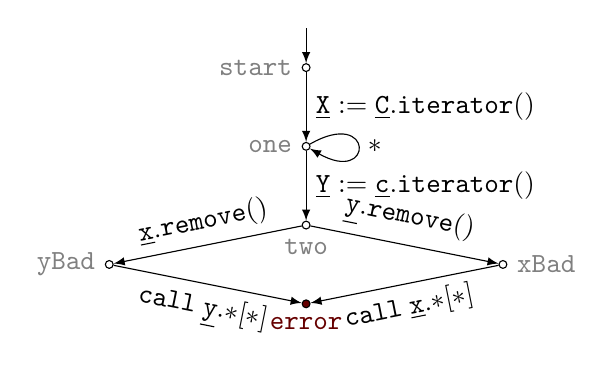
\begin{tikzpicture}
  \def\x{2.5}
  \tikzset{vertex/.style={draw,circle,inner sep=1pt}}
  \tikzset{transition/.style={->,>=latex}}
  \tikzset{every label/.style={gray}}
  \node[vertex] (start) at (0,0) [label=left:\texttt{start}] {};
  \node[vertex] (one) at (0,-1) [label=left:\texttt{one}] {};
  \node[vertex] (two) at (0,-2) [label=below:\texttt{two}] {};
  \node[vertex] (xBad) at (1*\x,-2.5) [label=right:\texttt{xBad}] {};
  \node[vertex] (yBad) at (-1*\x,-2.5) [label=left:\texttt{yBad}] {};
  \node[vertex,fill=darkred] (error) at (0,-3) [label=below:\textcolor{darkred}{\texttt{error}}] {};
  \draw[transition] (0,0.5)--(start);
  \draw[transition] (start)--node[right]{$\pattern X:=\pattern C.\mathtt{iterator}()$} (one);
  \draw[transition] (one) .. controls +(30:1cm) and +(-30:1cm) .. node[right]{$*$} (one);
  \draw[transition] (one)--node[right]{$\pattern Y:=\pattern c.\mathtt{iterator}()$} (two);
  \draw[transition] (two) -- node[sloped,above]{$\pattern y.\mathtt{remove}()$} (xBad);
  \draw[transition] (two)--node[sloped,above]{$\pattern x.\mathtt{remove}()$} (yBad);
  \draw[transition] (xBad)--node[sloped,below]{$\mathtt{call}\;\pattern x.{*}[*]$} (error);
  \draw[transition] (yBad)--node[sloped,below]{$\mathtt{call}\;\pattern y.{*}[*]$} (error);
\end{tikzpicture}
%\caption{A first example: Diagram of safety property}
%\label{fig:first.diagram}
%\end{figure}
%\begin{figure}
\begin{Verbatim}[commandchars=\\\{\}]
property InvalidateOtherIterators
  using prefix java.util.Collection
  using prefix java.util.Iterator
  start -> one:  \pattern{X} := \pattern{C}.iterator()
  one -> one:    *
  one -> two:    \pattern{Y} := \pattern{c}.iterator()
  two -> yBad:   \pattern{x}.remove()
  two -> xBad:   \pattern{y}.remove()
  yBad -> error: call \pattern{y}.*[*]
  xBad -> error: call \pattern{x}.*[*]
\end{Verbatim}
\caption{The property {\tt InvalidateOtherIterators} in diagram (left) and textual form (right).
}
\label{fig:first.topl}
\end{figure}
%
\begin{figure}
{\def\s#1{\text{\Verb@#1@}}
 \def\m#1{\PY{n+na}{#1}}
 \def\t#1{\mathtt{#1}}
\begin{align*}
&\{\;(\start,[])\;\} \\
&\s{Iterator<Integer> i = c.\m{iterator}();} \\
&\text{assume {\tt c} holds $1$, and {\tt i} holds $2$ } \\
& \begin{aligned}
  \{\;&(\start,[]),\\
      &(\t{one},[c:1,x:2])\;\}
  \end{aligned}\\
&\s{Iterator<Integer> j = c.\m{iterator}();} \\
&\text{assume {\tt j} holds $3$} \\
& \begin{aligned}
  \{\;&(\start,[]),\\
      &(\t{one},[c:1,x:2]),\\
      &(\t{one},[c:1,x:3]),\\
      &(\t{two},[c:1,x:2,y:3])\;\}
  \end{aligned}\\
&\s{i.\m{next}();} \\
& \begin{aligned}
  \{\;&(\start,[]),\\
      &(\t{one},[c:1,x:2]),\\
      &(\t{one},[c:1,x:3]),\\
      &(\t{two},[c:1,x:2,y:3])\;\}
  \end{aligned}\\
&\s{i.\m{remove}();} \\
& \begin{aligned}
  \{\;&(\start,[]),\\
      &(\t{one},[c:1,x:2]),\\
      &(\t{one},[c:1,x:3]),\\
      &(\t{yBad},[c:1,x:2,y:3])\;\}
  \end{aligned}\\
&\s{j.\m{next}()} \\
& \begin{aligned}
  \{\;&(\start,[]),\\
      &(\t{one},[c:1,x:2]),\\
      &(\t{one},[c:1,x:3]),\\
      &(\error,[c:1,x:2,y:3])\;\}
  \end{aligned}\\
\end{align*}}
\caption{A first example: Running step by step}
\label{fig:first.steps}
\end{figure} % >>>

\autoref{fig:first.steps} shows an execution of the program and of an automaton for the property \texttt{InvalidateOtherIterators}.
The lines \{in curly brackets\} describe the state of the automaton;
the lines in \texttt{monotype} show the statements that execute;
the other lines are comments.
At a given moment, the automaton has a set of active states.
A state is a pair of a vertex and a store.
The store is a memory that holds (automaton) variables.
Technically, it is a finite partial map from variables to values.
(A partial finite map is sometimes called a \emph{dictionary}.)

\begin{notation}
We write $[k_1:v_1,k_2:v_2]$ for the finite partial map that maps key~$k_1$ to value~$v_1$, and key~$k_2$ to value~$v_2$.
The empty map is denoted by~$[]$.
\end{notation}

The automaton has variables $x$,~$y$, and~$c$.
At vertex \texttt{one} the variables $x$~and~$c$ are initialized;
at vertex \texttt{two} the variables $x$,~$y$, and~$c$ are initialized.
Being at vertex \texttt{one} means that $x$~is an iterator for~$c$;
being at vertex \texttt{two} means that $x$~and~$y$ are two iterators for the same collection~$c$.
There is a program variable~\Verb@c@ and an automaton variable~$c$.
The same name was chosen because the two variables always hold the same value in this example.
In general, however, program variables and automaton variables live in different name-spaces, and may hold different values.

\begin{notation}
Program variables are typeset in \Verb@monotype@ (\Verb@c@,~\Verb@i@,~\Verb@j@).
Automaton variables are typeset in \textit{italics} ($c$,~$x$,~$y$).
Program variables appear in the program;
automaton variables do \emph{not} appear in the property.
Instead, automaton variable \emph{patterns} appear in the property, and they are typeset in \texttt{\underline{underlined monotype}} (\pattern c,~\pattern C, \pattern x, \pattern X, \pattern y,~\pattern Y).
\end{notation}

As it will become apparent below, the interaction between patterns and automatons' memory is as follows: uppercase patterns write to the automaton memory, and lowercase patterns read from the automaton memory and act as a guard on the transition.

\paragraph{Step~1.}

Initially, only the state $(\start,[])$ is active.
The outgoing transition of vertex \start is labeled by \[\pattern X:=\pattern{C}.\mathtt{iterator}()\] and the first executed statement is \verbline[.]{i = c.\PY{n+na}{iterator}()}
A method call matches a label when
\begin{itemize}
\item[(a)] the called method matches the method pattern, and
\item[(b)] the program values match their corresponding patterns.
\end{itemize}
By definition, any value matches an Uppercase pattern.
Here, the values of \Verb@i@~and~\Verb@c@ trivially match the patterns \pattern X~and~\pattern C.
The method itself also matches the method pattern, but for a slightly more complicated reason than it appears.
For simplicity, we ignore argument types and identify Java methods only by their fully qualified name and their arity.
The called method \texttt{iterator} is in the class \texttt{ArrayList} and has arity~$1$.
We identify it as follows.
\verbline{java.lang.ArrayList.iterator[1]}
Without \texttt{using prefix} directives, the method pattern would be \Verb@iterator[1]@.
With the directives, however, the pattern is the following.
\begin{align*}
&\text{\Verb@java.util.Collection.iterator[1]@} \\
&\text{\Verb@java.util.Iterator.iterator[1]@}
\end{align*}
It means that these two methods \emph{and} all those that override them match.
Here, \texttt{ArrayList} implements \texttt{Collection}.

All conditions are met to enable the transition from \start to \texttt{one}.
When the transition is performed the values that matched \pattern X~and~\pattern C are written in the automaton variables $x$~and~$c$.
For concreteness, let us assume these values are $1$~and~$2$.
After the transition is performed, the state $(\mathtt{one},[c:1,x:2])$ is active.
The state $(\start,[])$ remains active because the implicit transition \verbline{start -> start: *} is also enabled and performed.

\paragraph{Step~2.}
For the second step, the statement to be executed is \verbline[.]{j = c.\PY{n+na}{iterator}()}
Now we need to consider the two active states \[\{(\start,[])\quad\text{and}\quad(\texttt{one},[c:1,x:2])\}\] in turn.
For $(\start,[])$ the same reasoning as for step 1 holds, so the states $(\start,[])$ and $(\mathtt{one},[c:1,x:3])$ are active after step~2.
Note that now the automaton variable~$x$ remembers the value of the program variable~{\tt j}.
For $(\texttt{one},[c:1,x:2])$ we look at the transitions outgoing from vertex {\tt one}.
\begin{align*}
&\text{\Verb@one -> one: *@} \\
&\text{\Verb@one -> two: \pattern Y := \pattern c.iterator()@}
\end{align*}
The first of these transitions is always enabled, and performing it keeps states with vertex \texttt{one} active.
The second of these transitions has two patterns, \pattern Y~and~\pattern c.
The uppercase pattern~\pattern Y always matches;
the lowercase pattern \pattern c matches only the value held by the automaton variable~$c$.
In this case, the automaton variable~$c$ was set in the previous step to the value of the program variable~\texttt{c}.
Therefore, the transition from~\Verb@one@ to~\Verb@two@ is performed and the state $(\mathtt{two},[c:1,x:2,y:3])$ is activated.

\paragraph{Step~3.}

The third step involves the statement
\[\text{\Verb+\PY{n}{i}\PY{o}{.}\PY{n+na}{next}\PY{o}{(}\PY{o}{)}\PY{o}{;}+}\]
which matches no label of outgoing transitions of the currently active vertices (that is, \start, {\tt one}, and {\tt  two}).
Therefore, although the program proceeds, the set of active states of the automaton remains unchanged.

\paragraph{Step~4.}

In the fourth step, the transition $\texttt{two}\to\texttt{yBad}$ is performed.
Notice that the pattern $\pattern{x}.\mathtt{remove}()$ does not have a left-hand side, which simply means that the returned value is irrelevant for this transition.
The states corresponding to vertices \start and {\tt one} remain unchanged, because their outgoing transitions are disabled.
However,  the outgoing transition of state {\tt two} is enabled, and therefore {\tt yBad} becomes active.

\paragraph{Step~5.}

For the fifth and final step, the statement to be executed is \verbline[.]{j.\PY{n+na}{next}()}
The label of the outgoing transition  \[\mathtt{call}\;\pattern{y}.{*}[*]\] of the active state $(\texttt{yBad},[c:1,x:2,y:3]),$
has two distinguishing features: the~$*$ as a method name and the tag \texttt{call}.
As before, in order to match the method name, the following prefixes are prepended  
\begin{align*}
&\text{\Verb@java.util.Collection.*[*]@} \\
&\text{\Verb@java.util.Iterator.*[*]@}
\end{align*}
Then the $*$s are expanded, taking into account the \texttt{CLASSPATH}.
We have a match because the expansion \verbline{java.util.Iterator.next} is overridden by the method that is actually called.

The tag {\tt call} is used when we want the automaton to take a transition precisely at call-time of a method invocation.
The automaton expresses that a call to one of {\tt j}'s methods while vertex \texttt{yBad} is active constitutes an error.
Notice that this is different from a label like $\pattern X:=\pattern C.\mathtt{iterator}()$ which may match only after the return value is known.

\medskip
The execution we stepped through reaches the \error vertex, so we conclude that the property is violated.
Notice that in order to find a counterexample we need to keep track of the relation between several objects, in particular that iterators {\tt i} and {\tt j} are for the same collection {\tt c}.

% >>>
\subsection{More on Iterators} \label{sec:examples.iterators} % <<<

Other interesting properties of iterators~\cite{dblp:conf/oopsla/naeeml08,dblp:conf/sigsoft/boddenlh08,haack2009} are easily  to express in TOPL\null.

\medskip\emph{Modifying a collection invalidates all its existent iterators:}
\delimitVerbatim
\begin{Verbatim}[commandchars=\\\{\}]
property ModificationInvalidatesIterators
  using prefix java.util.Collection
  using prefix java.util.Iterator
  start -> iterating:    \pattern{I} := \pattern{C}.iterator()
  iterating -> modified: \pattern{c}.add(*), \pattern{c}.remove(*)
  modified -> error:     call \pattern{i}.*[*]
\end{Verbatim}
\delimitVerbatim
This property should list all the methods of \textit{Collection} that mutate it.
If classes that implement \textit{Collection} add mutating methods, then those should be included as well.
This abstraction leak is intrinsic to Java where sub-classing is not sub-typing.

\medskip\emph{Iterators should advance only if they are not exhausted:}
\delimitVerbatim
\begin{Verbatim}[commandchars=\\\{\}]
property UnsafeIteratorNext
  using prefix java.util.Collection
  using prefix java.util.Iterator
  start -> iterating:        \pattern{I} := *.iterator()
  iterating -> notExhausted: \pattern{true} := \pattern{i}.hasNext()
  notExhausted -> iterating: \pattern{i}.next()
  iterating -> error:        \pattern{i}.next()
\end{Verbatim}
\delimitVerbatim
The transition from \Verb@iterating@ to \Verb@notExhausted@ is enabled when \Verb@hasNext@ returns \Verb@true@.
In general, Java literals act as guards on transitions.

\medskip\emph{Method \Verb@remove@ may only be called after \Verb@next@:}
\delimitVerbatim
\begin{Verbatim}[commandchars=\\\{\}]
property RemoveBeforeNext
  using prefix java.util.Collection
  using prefix java.util.Iterator
  start -> created: \pattern{I} := *.iterator()
  created -> ok:    \pattern{i}.next()
  created -> error: \pattern{i}.remove()
\end{Verbatim}
\delimitVerbatim
TOPL is designed to track properties involving multiple objects.
However, properties involving a single object are also easy to express.
The vertex \Verb@ok@ is not special.
The purpose of the transition going to \Verb@ok@ is to deactivate the state with vertex \Verb@created@.

\medskip
We have now seen four properties of iterators.
Each of the previous TOPL properties corresponds to one English sentence.

\dinocomment{Maybe we need to add also the other example of the paper. Or put the other properties which are not related to iterators}

\section{TOPL Syntax and Semantics}


%\subsection{TOPL and iTOPL}\label{sec:syntax.topl} % <<<

%TOPL aims to be intuitive:
%Labels look like method calls, there is a shorthand notation for parallel transitions, there is an implied loop on the vertex \start, the \texttt{using prefix} directive offers some extra convenience, and so on.
%From the point of view of semantics, however, these conveniences are in the way.
%For this reason we also define iTOPL (\textbf inner TOPL), an even simpler language into which TOPL is desugared.

\autoref{fig:syntax.topl} shows the syntax of TOPL\null.
A property has a name, a set of \texttt{using} directives, and a set of transitions.
Each transition has an arc (directed edge) and labels.
Each arc has a source vertex and a target vertex.
All vertices are identified by their name.
Labels look like method calls.
Each label has a method pattern that is used to identify the set of methods to which the label refers.
In the simple case, a method pattern consists of a string pattern for the name of the method and an integer that specifies the method arity.
(For simplicity, TOPL does not use the static types of arguments to distinguish between overloaded methods.)
The more interesting case is when there are value patterns for each argument and perhaps even for the result.
Transitions should typically be tagged with \texttt{call} or \texttt{return} to specify exactly at what time they should be performed (see \autoref{sec:semantics.itopl} for details).
\dinocomment{Does anybody else has the ability to distinguish between call/return?}
%
\begin{figure}
\grammar{
  Property& \b{property} Identifier Using\* Transition\* \cr
  Using& \b{using prefix} StringPattern \cr
  Transition& Arc \b: Label \(\b, Label\)\* \cr
  StringPattern& \(Letter \| \b. \| \b*\)\+ \cr
  Arc& Vertex \b{->} Vertex \cr
  Label& Tag\? MethodPattern \cr
  Vertex& Identifier \cr
  Tag& \b{call} \| \b{return} \cr
  MethodPattern& ResultPattern\? NamePattern ArgumentsPattern \cr
  ResultPattern& ValuePattern \b{:=} \cr
  NamePattern& StringPattern \cr
  ArgumentsPattern& \b( \(ValuePattern \(\b, ValuePattern\)\*\)\? \b) \cr
  ArgumentsPattern& \b[ IntegerPattern \b] \cr
  ValuePattern& \b* \| Literal \| UppercaseId \| \b!\? LowercaseId \cr
  IntegerPattern& \b* \| IntegerLiteral \cr
}
\caption{Syntax of TOPL}
\label{fig:syntax.topl}
\end{figure}

There are three types of patterns used in TOPL---for strings, for integers, and for values.
String patterns are POSIX globs~\cite{man:glob.h} and match method names.
(For simplicity, TOPL does not use full regular expressions as string patterns.)
Integer patterns specify method arities.
Value patterns are the most interesting.
For each automaton variable \Verb@v@ there are three associated patterns.
The uppercase pattern \Verb@V@ matches any value and writes it in the automaton variable \Verb@v@.
The lowercase pattern \Verb@v@ reads the value of the automaton variable \Verb@v@ and only matches that value.
The negated lowercase pattern \Verb@!v@ reads the value of the automaton variable \Verb@v@ and only matches different values.
A Java literal acts as a pattern that matches only the value it denotes.
A wildcard~* pattern matches any value.

A TOPL property is \emph{well-formed} when it satisfies the following conditions.
\begin{itemize}
\item Labels must contain uppercase value patterns at most once.
\item Any use of a lowercase patterns must be preceded by a use of the corresponding uppercase pattern on all paths from the \start vertex.
  In other words, automaton variables must be written before being read.
\end{itemize}
It is easy to check that a property is well-formed~\cite{web:topl.prototype}.
From now on we assume TOPL properties to be well-formed.

%\paragraph{TOPL semantics}
%The TOPL formal semantics is defined by first mapping TOPL to  a simpler version of it (called iTOPL) with some restrictions (see~\cite{fool-paper} for details). In particular:
%\begin{itemize}
%\item Each transition has exactly one label.
%\item Each label is a list of (guard, action) pairs.
%\item Each guard is some boolean combination of atomic guards.
%\item Each action is a sequence of atomic actions.
%\item  An atomic guard that matches against method calls and always specifies a tag \Verb@call@ or \Verb@return@, but never involves examining any values.
%\end{itemize}
%These restrictions do not affect the expressivity of the language, rather they give us a more suitable  language for 
%a simpler formal development. 

\subsection{Semantics}\label{sec:semantics} % <<<

We consider a program's semantics to be a set of event traces.
Similarly, an automaton's semantics is also defined as a set of event traces.
We say that a program \emph{violates} a property when their sets of traces intersect.
In other words, properties encode bad executions, rather than good executions.

%\begin{notation}
%Sets are typeset in \set{SansSerif} with two exceptions---$\B$~is the set $\{0,1\}$, and $\N$~is the set $\{0,1,2,\ldots\,\}$.
%We write $\set A\times\set B$ for the set of all pairs $(a,b)$ with $a\in\set A$ and $b\in\set B$.
%We write $\set A\to\set B$ for the set of functions from~\set A to \set B.
%In particular, the powerset of~\set A is denoted by $\set A\to\B$.
%Note that $(\set A\to\set B)\subset\bigl((\set A\times\set B)\to\B\bigr)$.
%For all $f\in\set A\to\set B$, we write $f\;a$ or $f(a)$ to denote the unique~$b$ such that $(a,b)\in f$.
%We write $\set A\pmap\set B$ for the set of finite partial maps from~\set A to~\set B.
%Again, $(\set A\pmap\set B)\subset\bigl((\set A\times\set B)\to\B\bigr)$.
%However, there are functions that are not finite partial maps, and there are finite partial maps that are not functions.
%For all $f\in\set A\pmap\set B$, the domain $\{a\mid\text{$(a,b)\in f$ for some $b$}\}$ is finite.
%We write $f\;a$ or $f(a)$ only when $a$ is in the domain of~$f$.
%We write $\set A\,\mathsf{array}$ for $\bigcup_{n\in\N}
%\bigl(\{0,1,\ldots,n-1\}\to\set A\bigr)$.
%For $i\in\N$ and $a\in\set A\,\mathsf{array}$, we will usually write $a_i$
%instead of $a\;i$.
%\end{notation}

%\subsection{Semantics of iTOPL}\label{sec:semantics.itopl} % <<<
\begin{definition}
A TOPL property is a tuple $(\set{Vertex}, \set{Arc}, \set{Label}, \texttt{start}, \texttt{error})$ where
\begin{itemize}
\item $\set{Vertex}$ is a set of vertices;
\item $\set{Arc} \subseteq \set{Vertex} \times \set{Label} \times \set{Vertex}$ is a set of labelled arcs;
\item $\texttt{start} \in \set{Vertex}$ is the initial vertex;
\item $\texttt{error} \in \set{Vertex}$ is the accepting vertex.
\end{itemize} 
\end{definition}
Each TOPL's property gives rise to an automaton defined over the labeled multigraph  on $\set{Vertex}$ and $\set{Arc}$.
%$\set{Vertex}$ is the set of vertices mentioned as endpoints of the arcs and $\set{Arc}$ is the set of labeled arcs %mentioned in transitions. 
The automaton has two special vertices, {\tt start} and {\tt error}, the initial and accepting vertex respectively.

The automaton takes as input a trace of events.
Each event~$e$ contains an array of values.
Within guards and actions we write $e[i]$ for the $i$th value associated to event~$e$ (0-based).
We assume a countable set \set{Value} of values, a countable set \set{Event} of events with known arity,
and a countable set $\set{Variable}$ of automaton variables.
A {\em  automaton state} is not just a vertex but also a store: 
\[
\set{State} = \set{Vertex}\times\set{Store}
\]
That is, the state of the automaton is
given by specifying the vertex in the graph as well as the value of defined automaton variables.
%
We model stores as finite partial maps with finite domain.
\[
\set{Store} = \set{Variable} \pmap_{\mathit{fin}} \set{Value}
\]
%
A further consequence of the concept of transition depth is that the events to be received by  target states 
of different enabled transitions with different depth are
not the same.  For example for a trace of events $e_1 e_2 e_3\cdots$, if two transitions
turn out to be enabled, one with depth 2 and the other with depth 5,
then the end state of the first transition will see $e_3$, while the end state of the second transition $e_6$. 

For this reason, it is necessary to keep track
of which events are next to be received by each state during a run of
the automaton.

To formalize this bookkeeping, we introduce the notion of
\emph{execution state}. 
\newcommand{\World}{ExecState}
\[
\set{\World} = \set{State}\times\set{Trace}
\]
The first component records the state of the automaton (vertex
and store) and the second component records the remaining trace of
events for that state.
We can define a predicate that determines the possible execution state transitions
\[
\mathit{Step} \in \set{\World}\to\set{\World} \to \B
\]
This predicate is defined in \autoref{fig:adStep} and 
from it we can define a non-deterministic step function, where all
enabled transitions are performed:
\begin{align}
%\mathit{NdetStep}&\in(\set{\World}\to\B)\to(\set{\World}\to\B)\\
\mathit{NdetStep}&\in 2^{\set{\World}} \to 2^{\set{\World}}\\
%\mathit{NdetStep}\;S&=(\bigcup \mathit{Step})\;S \label{eq:ndetstep}
\mathit{NdetStep}\;S&=\{ s \mid \text{$\mathit{Step}(s', s)$ for some $s'\in S$} \} \label{eq:ndetstep}
\end{align}
An iterated version of \textit{NdetStep} is useful for defining reachable states.
We define it as the least fixed point for the following equation.
\begin{align}
\mathit{NdetStep}^\star\;S &= S \cup \mathit{NdetStep}^\star\;(\mathit{NdetStep}\;S)
\end{align}
%\rlp{Should this really include 0-sized steps?}
%\rg{I prefer to keep epsilon transition, unless there is a good reason to special-case them.}
Finally, we can define the set of traces described by an automaton:
\[
\{ e \mid
\exists\sigma'e',\;((\mathtt{error},\sigma'),e')\in\mathit{NdetStep}^\star\;\{((\mathtt{start},[]),e)\}
\}
\]
These are the traces that drive the automaton from the \texttt{start} vertex (with an empty store) to the \texttt{error} vertex.
\begin{figure}
\hbox to\hsize{\vbox{
\begin{alg}
\^  $\proc{Step}\;((x_1,\sigma_1),e_1)\;((x_2,\sigma_2),e_2)$
\=  ~if~ $e_2$ is not a suffix of $e_1$ ~then return~ $0$
\=  $e:=\text{$e_1$ without the suffix $e_2$}$
\=  ~for each~ transition $((y_1,y_2),l)$
\+    ~if~ $(y_1,y_2)\ne(x_1,x_2) \lor \mathit{len}\;l\ne\mathit{len}\;e$ ~then continue~
\=    $\sigma:=\sigma_1$
\=    ~for each~ $k\in 1\ldots\mathit{len}\;l$
\+      $(g,a):=l[k]$
\=      ~if~ $\lnot g(e_k,\;\sigma)$ ~then continue~ to line 3
\=      $\sigma:=a(e_k,\;\sigma)$
\-    ~if~ $\sigma=\sigma_2$ ~then return~ $1$
\-  ~return~ $\mathit{len}\;e=1\land\sigma_1=\sigma_2$
\end{alg}
\smallskip
}\hfil}
\caption{One automaton step}
\label{fig:adStep}
\end{figure}
\dinocomment{I think calling the traces $e_1$ and $_2$ is confusing with the events $e_k$.}


\paragraph{Deciding enabling of transitions.}
Given the state a peculiar aspect of our automata is deciding whether a transition is enabled.
Each label carries (potentially) a list of guards and 
we call the length of this list, the \emph{depth} of the transition.
%
In order for a transition to be enabled, all the guards along its
list have to evaluate to true. Since each guard along the transition consumes
an event |  therefore | if a transition has depth~$n$, then we have to examine the next~$n$ events to see if the transition is enabled.


We now describe when transitions are enabled. For this we have to look
at labels. A label is a list of pairs of guards and actions.
Let us look at guard first. A {\em general guard} is a partial function of type:
\[
\set{GenGuard} = (\set{Pattern} \times \N \times \set{Pred}) \pmap (\set{Event}\times\set{Store}) \to \B
\]
A general guard can be instantiated with a pattern  name, $\pattern v$,  its position $i$ in the label, and a predicate $p$ that we need to test this pattern for. By providing these arguments we obtained an {\em instantiated guard}:
\[
g_{\pattern{v},i,p} : \set{Event}\times\set{Store} \to \B
\]
that given an event and a store evaluate whether the event satisfy the guard in the store. It is defined as:
\newcommand{\sem}[1]{[ \! | #1 | \! ]}
\[
g_{\pattern{v},i,p}(e, \sigma) = p(e[i],\sigma(\pattern v))
\] that is the guard is true if and only if the value of $\pattern{v}$ in the automaton store 
and the value of $i$-th parameter of the event $e$ (which has been evaluated in the program store) satisfy $p$.
\begin{example}
Consider the label 
\[
 \sim \pattern {v}^0 := \pattern {s}^1 .gets(\pattern {k}^2)
 \] to be matched with event 
\[
 t^0:=z^1.gets(h^2)
\] the upper-script stands for the position of a pattern or an expression. In this case we want to compare: 
$\pattern{v}$ against  $t$, $\pattern s $ against $z$, and $\pattern k$ against $h$. Notice that the predicates we want to compare for are equality for the element in position 1 and 2, but inequality for position 0 (because of $\sim$).
Hence, the instantiated guards are: $g_{\pattern{v},0, \neq}$, $g_{\pattern{s},1,=}$, and $g_{\pattern{k},2,=}$. 
Before matching, the pattern is compiled down to the sequences 
\[
\pattern{call} \  \pattern{s}^0 .gets(\pattern {k}^1);  \ \pattern{ret} \ gets = \sim \pattern {v}^0   
\] generating the instantiated guards: 
$g_{\pattern{v},0, \neq}$, $g_{\pattern{s},0,=}$, and $g_{\pattern{k},1,=}$ to be matched with events $e_1;e_2$ 
where
\[ 
 e_1=(call \ gets, [0: \sem{z}, \ 1: \sem{h}])  \quad \mbox{ and }  \quad e_2= (ret \ gets, [0: \sem{t}])  
\]  generated out of the statement. This is done by taking the conjunction of guards:
\[ 
 (tag(e_1)= \ call \ gets) \wedge g_{\pattern{s},0,=}(\sigma,e_1) \wedge g_{\pattern{k},1,=}(\sigma, e_1) 
\] and 
\[ 
 (tag(e_2)= ret \ gets) \wedge g_{\pattern{v},0,\neq}(\sigma,e_2).
\]
\end{example}

%A guard compares the values in an event with those in a store and
%concludes either pass or no pass:
%\[
%\set{Guard} =\set{Event}\times\set{Store} \to \B
%\]



If the event passes a guard, the corresponding action is performed on that event.
Actions modify the store, using values from an event:
\[
\set{Action} = \set{Event}\times\set{Store}\to\set{Store}
\]
In order for a transition of depth $n$ to be enabled for a trace of
events, the first $n$~events of the trace must pass the $n$~guards
on the label with the stores modified by the guards:
\[
\begin{array}{c l}
& \enabled((g_1, a_1), \ldots, (g_n, a_n); e_1, \ldots, e_n; s) \\
 = &
g_1(e_1, s_0)\ \land\ \ldots\ \land\ g_n(e_n, s_{n-1}) 
\end{array}
\]
where
\begin{align}
  s_0 &=  s \\
  s_i &= a_i(e_i, s_{i-1}) &&\text{for $i\in1.\,.\,n$}
\end{align}
The store for the target vertex of enabled and performed transition will be $s_n$.

\paragraph{Silent steps.}
Another peculiar aspect of our
automatons is that if no transitions are enabled for a given
state and trace of events, the automaton does not get stuck but is
allowed to consume one event without changing its state (called a silent step). Note that
a silent step is not equivalent to an implied self-loop on all states, as
dropping events is not allowed if there are any enabled
transitions. In that case one of the enabled transitions is performed and
the automaton execution state becomes $((v, s_n), \mathit{events}_n)$, where $v$ is the vertex at the
end of the arc of the transition, $s_n$ is defined as above and
$\mathit{events}_n$ is the current executions state's event trace with the first
$n$ events dropped.
\begin{example}
Consider the two automata in Figure~\ref{fig:unmatched-example} and assume that the set of active states for the left-hand side automaton is $\{ \texttt{zero} \}$ and for the right-hand side one is $\{ \texttt{three}\}$. Moreover, let us assume we are given the following
trace in input
\[
\cdots e_1 e_1 e_2 \cdots
\] In the left-hand side automaton, the first occurrence of the event $e_1$ enables the transition  from {\tt zero} to {\tt two}, however, the transition from {\tt zero} to {\tt one} cannot fire since the first occurrence of $e_1$ is followed by another $e_1$.
Consequently, after the first occurrence of $e_1$ state {\tt two} becomes active and {\tt zero} inactive. 
Notice that, in the left-hand side automaton, state {\tt one} cannot be reached by 
the trace $e_1 e_1 e_2 $ from {\tt zero}. 
On the contrary, for the right-hand side automaton, the first occurrence of $e_1$ does not enable any transition per se. 
Notice that the only outgoing transition on the active state {\tt three} needs a sequence of two events to be enabled. Hence, we need to consider the sequence $e_1e_1$. The latter does not enable any transition either. Therefore, according to our semantics,  the first occurrence of $e_1$ is consumed silently and the set of active states (i.e., $\{ \texttt{three} \}$) remains unchanged. At this point, the second occurrence of $e_1$ is considered, and since it is followed by $e_2$ the transition from {\tt three} to {\tt four} becomes is enabled, the events $e_1e_2$ are consumed and {\tt four} becomes active whereas {\tt three} inactive.
\end{example}
\begin{example}
Consider {\em Step 3} in Section~\ref{}. The event produced by the statement 
\[\text{\Verb+\PY{n}{i}\PY{o}{.}\PY{n+na}{next}\PY{o}{(}\PY{o}{)}\PY{o}{;}+}\] 
is not matched by any transitions starting from states {\tt one} or {\tt two} in the automaton of Fig~\ref{}. 
This event is silently consumed but the set of active states does not change. 
The automaton will take a transition as soon as a suitable event matching an outgoing transition of an active state is encountered in the trace.
\end{example}
%
%
\begin{figure}
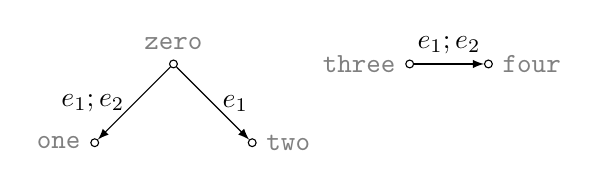
\begin{tikzpicture}
  \def\x{2.5}
  \tikzset{vertex/.style={draw,circle,inner sep=1pt}}
  \tikzset{transition/.style={->,>=latex}}
  \tikzset{every label/.style={gray}}
  \node[vertex] (zero) at (0,0) [label=above:\texttt{zero}] {};
  \node[vertex] (one) at (-1,-1) [label=left:\texttt{one}] {};
  \node[vertex] (two) at (1,-1) [label=right:\texttt{two}] {};

  \node[vertex] (three) at (3,0) [label=left:\texttt{three}] {};
  \node[vertex] (four) at (4,0) [label=right:\texttt{four}] {};
  
  \draw[transition] (zero)--node[left]{$ e_1;e_2$} (one);
  \draw[transition] (zero)--node[right]{$e_1$} (two);
  
  \draw[transition] (three)--node[above]{$e_1;e_2$} (four);
\end{tikzpicture}
\caption{Example of unmatched events.}
\label{fig:unmatched-example}
\end{figure}

% >>>
%\subsection{Semantics of SOOL} \label{sec:semantics.sool} % <<<

%The \emph{program state} holds method parameters and dynamically allocated objects.
%Method parameters are held in a store;
%dynamically allocated objects are held in the heap.
%The \emph{heap} is a finite partial map from (object reference, field name) pairs to values.
%\begin{align}
%\set{SoolState}&=\set{Store}\times\set{Heap}\\
%\set{Store}&=\set{Variable}\pmap\set{Value} \\
%\set{Heap}&=(\set{Value}\times\set{Variable})\pmap\set{Value}
%\end{align}
%The input is a stream of values;
%the output is an array of events.
%The \emph{program world} keeps track of the program state, the input yet to be consumed, and of the output already produced.
%\begin{align}
%\set{Input}&=\N\to\set{Value} \label{eq:input}\\
%\set{Trace}&=\set{Event}\,\mathsf{array} \\
%\set{SoolWorld}&=\set{SoolState}\times\set{Input}\times\set{Trace} \\
%((\sigma, h), i, o)&\in\set{SoolWorld} \label{eq:epstate.element}
%\end{align}
%Equation~\eqref{eq:epstate.element} shows the general form of an element of~\set{SoolWorld}: $\sigma$~is the store that holds parameters, $h$~is the heap that holds dynamically allocated objects, $i$~is the input stream yet to be processed, and $o$~is the array of events already emitted.
%The implementation~\cite{web:topl.prototype} also has local variables, which are treated similarly to method parameters.

%Executing a SOOL program amounts to executing the \Verb@main@ body, which is a compound statement.
%\begin{align}
%\mathit{exec}&\in(\set{SoolWorld}\times\set{Statement})\to(\set{SoolWorld}\times\set{Value})
%\end{align}
%Method calls are interesting.
%The general form of a method call is \[ e.x := f.m(g_1,\ldots,g_n)\] where $e$,~$f$, $g_1$, \dots, $g_n$ are expressions, $x$~identifies a data field, and $m$~identifies a method.
%Expressions evaluate to values and do not have side-effects.
%\begin{align}
%\set{Expression}&=\set{SoolState}\to\set{Value} \\
%e,f,g_1,\ldots,g_n&\in\set{Expression}
%\end{align}

%\begin{notation}
%The map $\sigma[k:v]$ is the same as the map~$\sigma$, except it maps $k$~to~$v$.
%\end{notation}

%\autoref{fig:exec.call} shows the definition of \textit{exec} for method calls.
%In spite of the imperative-looking notation, there is no mutation:
%Different versions of $\sigma$,~$h$, $i$, and~$o$ get different indices.
%Line~1 introduces a shorthand notation for the program state~$s$.
%Line~2 looks up in the program text a method named~$m$.
%We assume that method names are unique.
%The formal parameters of~$m$ are $x_1$,~\dots,~$x_n$.
%We assume a type-checker enforces that all calls are made with the correct number of arguments.
%The body of~$m$ is~$b$.
%Line~3 constructs a store that maps formal arguments to the actual values;
%$\sigma_1$~is commonly called the \emph{call stack frame} of~$m$.
%Line~4 emits the first event:
%It has tag $\mathtt{call}m$ and carries the actual argument values.
%Line~5 executes the body, by calling \textit{exec} recursively.
%Line~6 emits the second event:
%It has tag $\mathtt{return}m$ and carries the return value.
%Line~7 stores the return value in the heap.
%Finally, line~8 returns the updated program execution state and the unit value~$()$.

%\begin{figure}
%\hbox to\hsize{\vbox{
%\begin{alg}
%\^  $\proc{exec}\Bigl(\bigl((\sigma_0,h_0),i_0,o_0\bigr),\bigl(e.x:=f.m(g_1,\ldots,g_n)\bigr)\Bigr)$
%\=  $s:=(\sigma,h)$
%\=  $((x_1,\ldots,x_n), b) :=\mathit{methodOfName}\;m$
%\=  $\sigma_1:=[\textbf{this}:(f\;s), x_1:(g_1\;s), \ldots, x_n:(g_n\;s)]$
%\=  $o_1:=\text{$o_0$ with $(\mathtt{call}m,[f\;s,g_1\;s,\ldots,g_n\;s])$ appended}$
%\=  $(((\sigma_2,h_2),i_2,o_2),v):=\mathit{exec}\bigl(((\sigma_1,h_0),i_0,o_1),b\bigr)$
%\=  $o_3:=\text{$o_2$ with $(\mathtt{return}m,[v])$ appended}$
%\=  $h_3:=h_2[(e\;s, x) : v]$
%\=  ~return~ $(((\sigma_2,h_3),i_2,o_3), ())$
%\end{alg}
%\smallskip
%}\hfil}
%\caption{Executing one SOOL method call}
%\label{fig:exec.call}
%\end{figure}

%Other statements are interpreted as usual and are not interesting.

%Given a program with the main body~$b$, the output trace~$o$ corresponding to some input~$i$ is obtained by starting the execution with an empty store~$[]$, an empty heap~$[]$, and an empty output~$[]$.
%\begin{align}
%((\_,\_,o),\_):=\mathit{exec}\bigl((([],[]),i,[]),b\bigr)
%\end{align}



\section{Run-time checking}
In this section we describe an algorithm to at run-time TOPL properties on Java programs.

Figure~\ref{architecture} summarises our method. There are two main components: the {\em TOPL compiler} and the {\em Property Checker}.  
The TOPL compiler takes in input the compiled class files and the list of TOPL properties to be checked against the classes. The compiler has two submodules: the {\em instrumentator} and the {\em automaton generator}.
The automaton generator synthesises a Java program that precisely encode the set of automata representing the TOPL properties. The instrumentator instruments the byte code with calls to methods of the Java encoding of the automata.
During their tasks, the two submodules need to exchange information about method identifiers, therefore the two operations are intertwined.   
The property checker module can be seen as a general interpreter able to execute TOPL automata properties. When compiled together with the Java encoding of the automata generated by the TOPL compiler, we obtain an executable property checker instantiated to the particular list of TOPL properties we want to check against the initial class files.
When run together with the instrumented class files, the instantiated property checker acts as a monitor that is able to detect violation of the properties of interest.

In the following we give a detailed description of the TOPL compile and the Property checker.
\dinocomment{to myself: what's the difference with Polymer?}
%
\begin{figure}[htbp]
\begin{center}
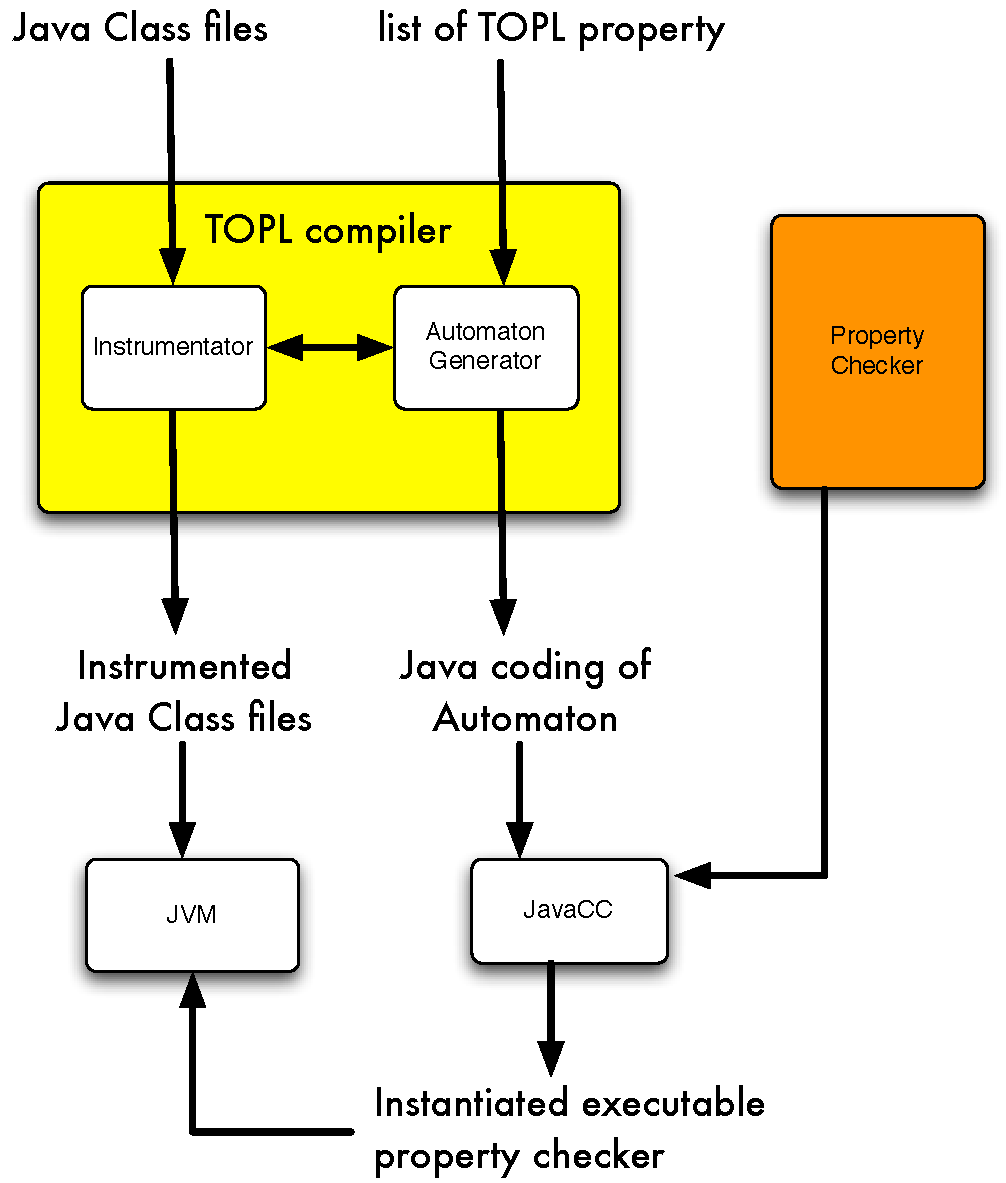
\includegraphics[scale=.35]{TOPL.pdf}
\caption{Architecture of TOPL properties' run-time checking.}
\label{architecture}
\end{center}
\end{figure}


\subsection{Run-time completeness}
\dinocomment{Rewrite in term of "security".}
A legitimate question about our run-time checker is whether it is {\em complete}. Informally, that can be expressed as:
\begin{quote}
if any run-time execution of the program leads to an error then will the checker detect the error?
\end{quote}
The program in Figure~\ref{fig:completeness} shows that in order to achieve completeness any run-time checker would need an unbound amount of memory. The method {\tt NeedsUnboundMemory(int n)}  declares an array of iterators of length depending from the external parameter {\tt n}.  In the {\tt for} loop, the array is filled with iterators of the same collection {\tt c} and randomly some of them  are exhausted by advancing them till the end (inner {\tt while} loop).
Outside the {\tt for} loop, a random iterator is advanced one more time and we would get  and exception if this iterator 
was  one of those exhausted in the previous loop. Because of the random choice of iterators, it becomes apparent that, 
if we were to decide at {\tt a[r.nextInt(n)].next()} whether an exception need to be thrown or not we would need to keep information about all the iterators. Moreover, since their number {\tt n} is a parameter, there is no way to bound the amount of memory this checker would need for keeping track of all the iterators. Therefore we conclude that any run-time checker would need {\em unbound memory} to detect whether this program gives an exception or not. 
%
\begin{figure}[htbp]
\begin{center}
\begin{Verbatim}[commandchars=\\\{\}]
\PY{k+kn}{import} \PY{n+nn}{java.util.*}\PY{o}{;}
\PY{k+kd}{public} \PY{k+kd}{class} \PY{n+nc}{Completeness} \PY{o}{\PYZob{}}
   \PY{n}{Collection} \PY{n}{c}\PY{o}{;}
   \PY{n}{Random} \PY{n}{r}\PY{o}{=}\PY{k}{new} \PY{n}{Random}\PY{o}{(}\PY{o}{)}\PY{o}{;}
   \PY{k+kd}{public} \PY{k+kt}{void} \PY{n+nf}{NeedsUnboundMemory}\PY{o}{(}\PY{k+kt}{int} \PY{n}{n}\PY{o}{)} \PY{o}{\PYZob{}}
      \PY{n}{Iterator}\PY{o}{[}\PY{o}{]} \PY{n}{a} \PY{o}{=} \PY{k}{new} \PY{n}{Iterator}\PY{o}{[}\PY{n}{n}\PY{o}{]}\PY{o}{;}
      \PY{k}{for} \PY{o}{(}\PY{k+kt}{int} \PY{n}{i}\PY{o}{=}\PY{l+m+mi}{0}\PY{o}{;} \PY{n}{i}\PY{o}{<}\PY{n}{n}\PY{o}{;} \PY{n}{i}\PY{o}{+}\PY{o}{+}\PY{o}{)} \PY{o}{\PYZob{}}
          \PY{n}{a}\PY{o}{[}\PY{n}{i}\PY{o}{]}\PY{o}{=}\PY{n}{c}\PY{o}{.}\PY{n+na}{iterator}\PY{o}{(}\PY{o}{)}\PY{o}{;}
          \PY{k}{if} \PY{o}{(}\PY{n}{r}\PY{o}{.}\PY{n+na}{nextBoolean}\PY{o}{(}\PY{o}{)}\PY{o}{)} 
	    \PY{k}{while} \PY{o}{(}\PY{n}{a}\PY{o}{[}\PY{n}{i}\PY{o}{]}\PY{o}{.}\PY{n+na}{hasNext}\PY{o}{(}\PY{o}{)}\PY{o}{)} \PY{n}{a}\PY{o}{[}\PY{n}{i}\PY{o}{]}\PY{o}{.}\PY{n+na}{next}\PY{o}{(}\PY{o}{)}\PY{o}{;}	
      \PY{o}{\PYZcb{}}\PY{o}{;}
      \PY{n}{a}\PY{o}{[}\PY{n}{r}\PY{o}{.}\PY{n+na}{nextInt}\PY{o}{(}\PY{n}{n}\PY{o}{)}\PY{o}{]}\PY{o}{.}\PY{n+na}{next}\PY{o}{(}\PY{o}{)}\PY{o}{;}
  \PY{o}{\PYZcb{}}\PY{o}{;}
\PY{o}{\PYZcb{}}
\end{Verbatim}

\caption{Counterexample to run-time completeness.}
\label{fig:completeness}
\end{center}
\end{figure}

\dinocomment{discuss about: conservative and transparent properties of an inliner}
\dinocomment{talk about our strategy}
\subsection{Checker}
\subsection{Byte code instrumentation}

\section{Experimental Results}

\dinocomment{experiments: TOMCAT, ANT, Eclipse and Dacapo benchmarks}

% >>>
\section{Related Work}\label{sec:related} %<<<
Our work is based on the concept of typestate~\cite{strom1986} originally developed for imperative programs and extends this fundamental concept by integrating notions typical of object-oriented programs. 
We are certainly not the first in doing this: there are several extensions of typestate to object-oriented programming in the literature.
A modular static verification method for typestate protocols is introduces in~\cite{dblp:conf/oopsla/bierhoffa07}. 
The specification method is based on linear logic and relations among objects in the protocol are monitored by a tailored system of permissions. 
The method is highly modular and presumably efficient. The specification of the interactions among objects by means of permissions adds an extra level of machinery which increases the gap between the intuitive protocol description and its formalization. Similarly~\cite{deline2004,dblp:conf/sigsoft/BierhoffA05} provide a mean to specify typestate properties that belong to a single object. The specified properties are reminiscent of contracts or pre/post-conditions for methods and
can deal with inheritance.
In~\cite{dblp:conf/issta/FinkYDRG06} the authors present sound verification techniques for typestate properties of Java  programs.
Their approach is divided in several stages with different verifiers varying for cost and precision.
In the early stages efficient but imprecise analyses are employed whereas
more expensive and precise techniques are then progressively employed in later stages.
Every stage focuses on verifying only the parts of the code that previous stages failed to verify.
It is likely that our TOPL language could be fruitfully combined with their analysis technique.

An automaton-based formalism for specifying properties of software interfaces were introduced in~\cite{dblp:conf/sigsoft/AlfaroH01} . 
This language aims at capturing assumptions about the order in which the methods of a component are called and the order in which the component calls external method.
In contrast to \TPL, this formalism is mainly used to check the compatibility of the interfaces of two components and it is designed to be applied at  model level rather than code level. A specification language for interface checking aimed to C programs (called SLIC) is introduced in~\cite{ball2002}.  
Differences between SLIC and \TPL \ include: the use (in SLIC) of
non-determinism to encode universal quantification of dynamically allocated data, and the  ability to have complex code in the automaton transitions. 
\TPL \ specifications naturally express universally quantified
properties over data structures and for computability reasons,  we
have chosen to limit the  actions performed during automaton transitions. 
Simple SLIC specifications are verified by  the SLAM verifier~\cite{dblp:conf/cav/ballr01}.
While SLAM specialises on device drivers and checks client conformance rather than full protocols, 
very general specifications of object-oriented program behaviour can be given in JML~\cite{jml} and Spec$\sharp$~\cite{DBLP:journals/jot/BarnettDFLS04}. However the latter two languages focus on class specifications and do not have temporal features.

In~\cite{disney2011} contracts are used to express legal traces of
programs in a functional language with references. The contracts
specify traces as regular expressions over calls and returns and so
look similar to our automatons, if for a quite different
setting. Here, the specifications are function-centered, though, and
again, capturing inter object relations seems somewhat awkward.

\dinocomment{Add more on dynamic checks and byte code instrumentation}

% >>>
\section{Conclusions and Future Work}\label{sec:conclusions} %<<<

\paragraph{}
We introduced TOPL---a language for expressing temporal safety properties for object-oriented programs.
TOPL properties can express constraints involving the relation of many objects at the same time. 
Furthermore, we introduced a technique for checking at run-time the violation of the properties
on Java program. We have applied our technique to a variety of programs including large open source Java projects.
%
\paragraph{Future work.}
In the future, we intend to make use of separation logic~\cite{reynolds2002} to deal with the heavy use of the heap and aliasing in object-oriented software. Moreover, we aim at developing static analysis techniques for \TPL \ properties of Java programs using the jStar framework~\cite{DBLP:conf/oopsla/DistefanoP08}.
This will require investigating suitable abstraction techniques for obtaining meaningful and precise over-approximations of the state space of the programs.
Finally, we intend to develop a tailored bi-abduction inference technology~\cite{dblp:conf/popl/CalcagnoDOY09} which would help with scalability of the analysis.
\dinocomment{Mention that we want to at least reach runtime soundness with abstractions}


%>>>

%\softraggedright
\bibliographystyle{IEEEtran}
\bibliography{safety}
\end{document}
% vim:spell errorformat=%f\:%l-%m,%f\:%l\:%m,%f\:%m
% vim:fmr=<<<,>>>:
